\documentclass{article}
\usepackage{graphicx}
\graphicspath{ {./images/} }
\begin{document}


\title{\textbf{Lab 6 Assignment}}
\author{\texttt{2019-CE-39 [USHNA IJAZ]}}
\maketitle

\section*{Question 1}
In this exercise, we will explore different types of randomized algorithms. We say that a
randomized algorithm is a Las Vegas algorithm if it is always correct (that is, it returns
the right answer with probability 1), but the running time is a random variable. We say that
a randomized algorithm is a Monte Carlo algorithm if there is some probability that it is
incorrect. For example, QuickSort (with a random pivot) is a Las Vegas algorithm, since it
always returns a sorted array, but it might be slow if we get very unlucky.
We will revisit the Majority Element problem to get more insight on randomized
algorithms.
\begin{center}
\begin{tabular}{|c|p{3cm}|p{3cm}|p{3cm}|p{3cm}|}
\hline
\textbf{Algorithm} & \textbf{Monte Carlo or Las Vegas?} & \textbf{Expected Running Time}
& \textbf{Worst-case Running Time} & \textbf{Probability of returning a majority element} \\
\hline
\textbf{Algorithm 1} & Las Vegas & O(n) & O(1) & 1 \\
\hline
\textbf{Algorithm 2} & Monte Carlo & O(n) &O(n) &$[\ge 1 – (1/2)^{100}]$ \\
\hline
\textbf{Algorithm 3} &Las Vegas &O(n) &$O(n^2)$ & 1 \\
\hline
\end{tabular}
\end{center}
\begin{flushleft}

\textbf{Answer}:
Short justification for each entry of the
table.
\linebreak 

\emph{First Algorithm:} This is Las Vegas.  A Las Vegas algorithm for this task is to keep picking a random element until we find a 1. The code in Algorithm 1 shows us a variable p which is generated randomly. If isMAJORITY contains the values of P, then p is returned; otherwise, the algorithm repeats this process until it finds the answer. isMajority takes time O(n) \textbf{ so the running time is O(n)}. The probability of returning a majority element here will be 1, because the algorithm will always return a majority element.
\linebreak 

\emph{Second Algorithm:} This is Monte Carlo. For a Monte Carlo algorithm with one-sided errors, the failure probability can be reduced by running the algorithm k times. This is Monte Carlo because it might return P[0], which may not be an majority element.
P. The number of iterations here are 100. Each iteration takes time O(n), so the
worst-case running time is O(n). The Monte Carlo Algorithm finds a 1 with probability $1 – (1/2)^k$
\linebreak 

\emph{Third Algorithm:} Algorithm is Las Vegas and is very similar to algorithm 1.  it iterates over all the elements, and so it will eventually hit a majority element, which it will return.

\section*{Question 2}

[Counting Inversions]: Given an array A of n elements, we call (i, j) an inversion if $0 \le I < j < n and A[i] > A[j].$\\
(a) Describe an $O(n^2)$ algorithm to count the number of inversions in a given array.

\textbf{Description}: For each element we count all elements less than  to its right and then add to the count to the final answer. The complexity is $O(n^2)$. Python Implementation:

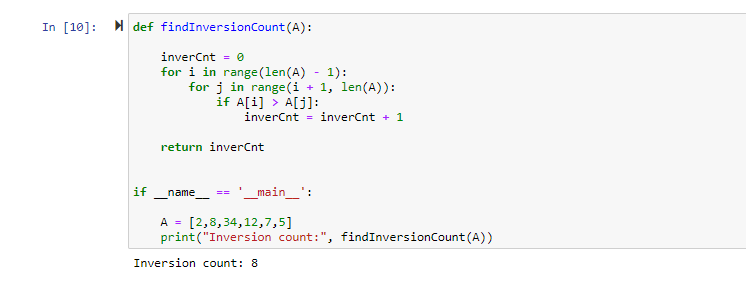
\includegraphics{q2lab6}

(b) Describe an O(n*log(n)) algorithm to count the number of inversions in a given array.
[Hint: Think about how you can modify MergeSort to solve this problem.]
[We are expecting: Actual code, and a short English description explaining the main idea
of the algorithm. We are also Expecting an informal justification of correctness and of the
running time.]
\linebreak 
\textbf{Answer}: The idea is similar to merge sort, divide the array into two equal or almost equal halves in each step until the base case is reached.\\
In the merge stage, two sorted arrays are merged into one sorted array. The main idea is to count the number of split inversions in a list (that is, where an element in the first half of the unsorted list should appear after a given element in the second half of the unsorted list. Then the number of split inversions involving an element  of the second array is precisely the number elements lefts in the first array. At the end we just add up the split inversions.
The algorithm used is divide and conquer, So in each level one full array traversal is needed and there are log n levels so the time complexity is O(n log n).\\
\textbf{$T(n) = 2T(n/2) + O(n)$}


\section*{Question 3} [Unified Duck Problem] Suppose that the n ducks are standing in a line. Each duck has
a favorite activity: honking, eating, or simply doing nothing (idling). And since they are
ducks, they do whatever they like to do all day long. You’d like to sort the ducks so that
all the honking ducks are on the left, the eating ducks are on the right, and the idling ducks
are in the middle*. You can only do two types of operations on the ducks:
\linebreak 

(a) Design an algorithm to sort the ducks which takes $O(n)  $ seconds and requires you to remember no more than seven integers between 0 and n-1	at a time.
[We are expecting: Pseudocode AND a short English description of your algorithm.]\\

\textbf{Answer:}
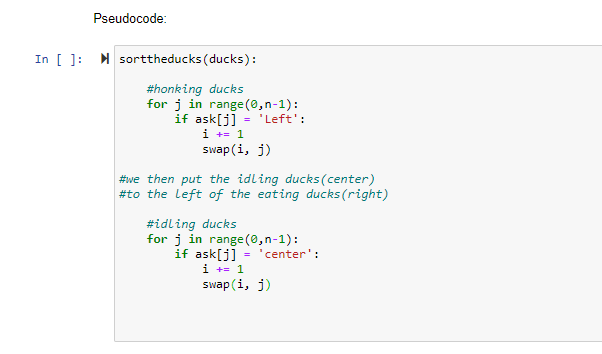
\includegraphics{q3a}
Description: This pseudocode was designed with the help of the quicksort algorithm. In the first loop, the algorithm puts the honking ducks(left) on the left and the rest will be sorted to the right. The second loop will swap the center ducks with those of the right. In the second loop all of the ducks that are left of the position \textit{i} will be sorted (left or center). The ducks left will be to the right of the position \textit{i}. Thus, sorted.
\linebreak 
(b) Justify why your algorithm is correct, why it takes only O(n) seconds, and why it
requires you to remember no more than seven integers at a time.
\linebreak 
\textbf{
Answer:} This algorithm uses two loops and as told in the question it uses 2 operations: ask(j) and swap(i,j) so the total cost is 4n.\\

Correctness: 
We assume that the recursive calls work correctly. Then, two halves of the array are sorted. Consider two elements i < j. For the base case, i and j=0. We assume it is true when i-1 so then when ith element is a honking duck (left) we swap  with j's position. Before the swap operation it was on the left so now we get 0 to j ducks are honking duck (left). Thus, when our first loop ends, there are no
left-leaning ducks left among i, . . . , n-1 After the incremental step we advance to the next loop. The same goes for the second loop, except it puts the center ducks to the left of the right ducks. At the end, all the ducks are sorted.
\end{flushleft}
\end{document}